\chapter{Results, Analysis and Evaluation}

\setlength{\epigraphwidth}{0.43\textwidth}
\epigraphhead[50]{\epigraph{\large{`One molecule of \ce{H2O} is not wet;\\ only a
collection of molecules at some point has the property of wetness'}}{- Marcus du
Sautoy\\
The Creativity Code}}

\section{Testing the simulation}
\label{Testingthesimulation}

Simulation testing was performed experimentally, where observed results were
compared to expected results for any given piece of simulation functionality. In
a project with a larger dedicated pool of resources, 
a more robust testing strategy could have involved co-simulating; the
network simulation would be run alongside a mathematical abstraction that holds
assertions on states in the network, alerting the user when those assertions
are broken.

\subsection{Example of a simple spiking network}

As seen in the first example topology in the previous chapter, figure
\ref{fig:top1}, the simplest arrangement of neurons is a single synapse with a
pre and post synaptic neuron. The membrane potentials of the simulation of such
an arrangement can be seen in figure \ref{fig:PRERES1}. The exponential decay of
the synaptic connection can be observed as the "humps" in the post-synaptic
neuron's membrane potential in orange.

\begin{figure}[h!]
    \centering
    % \addtolength{\leftskip} {-4cm}
    % \addtolength{\rightskip}{-4cm}
    % 
\includegraphics[width=0.06\linewidth]{figures/tops/topexamrestwo.png}\vspace{-3ex}
    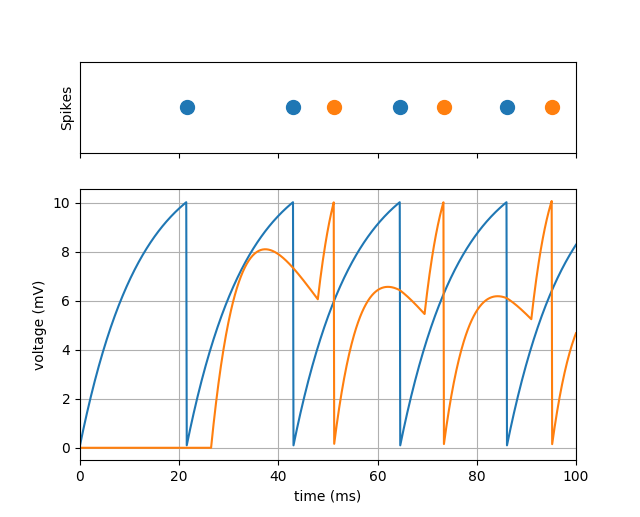
\includegraphics[width=0.7\linewidth]{figures/graphs/DelayBugFixed.png}
    \caption[A simple two-neuron network]{A simple two-neuron network. The input neuron (blue) fires under a constant input current. The second neuron (orange) is synaptically linked, and the synapse has a arbitrary delay of 5ms.}
    \label{fig:PRERES1}
\end{figure}
\FloatBarrier
In order to meet the requirement set out previously in chapter 3, section
\ref{SimulationRequirements}, for the availability of noisy inputs in a
simulated network, the input current of the pre-synaptic neuron can be drawn
from a random distribution, as shown in figure \ref{fig:PRERES2}. 

\begin{figure}[h!]
    \centering
    % \addtolength{\leftskip} {-4cm}
    % \addtolength{\rightskip}{-4cm}
    % 
\includegraphics[width=0.06\linewidth]{figures/tops/topexamrestwo.png}\vspace{-3ex}
    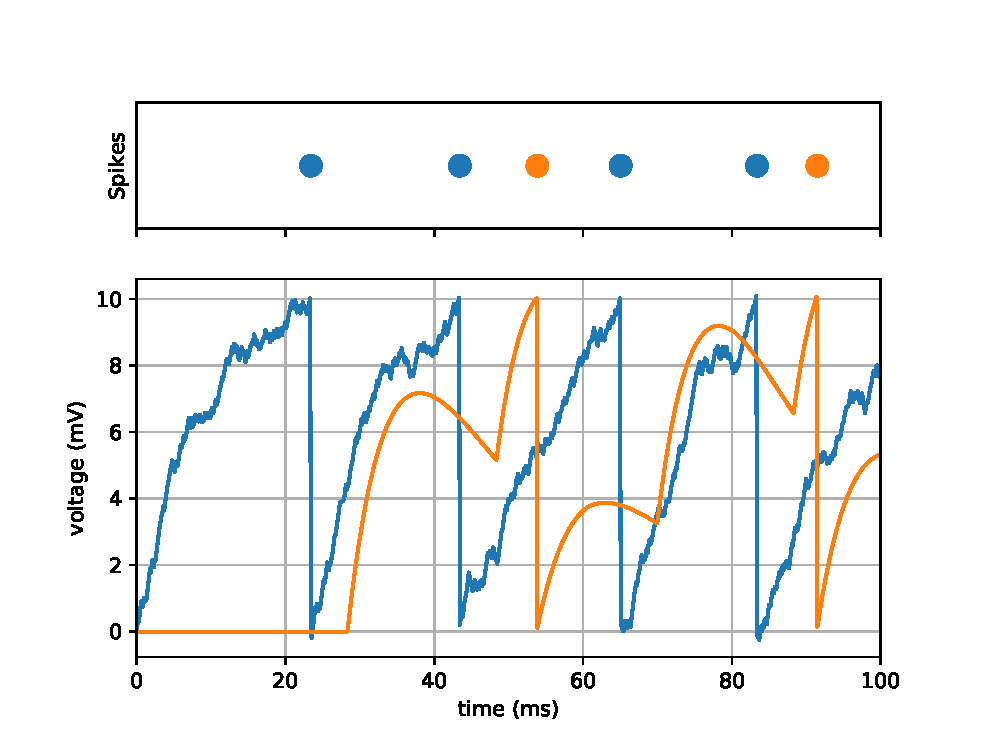
\includegraphics[width=0.7\linewidth]{figures/graphs/twospikingneuronsdelaynoise.eps}
    \caption[A simple two-neuron network with noise]{A simple two-neuron network, with a noisy input. The input current to the pre-synaptic neuron (blue) is drawn from a normal distribution, so the average time between spikes is the same as can be observed in \ref{fig:PRERES1} overall. The spiking pattern of the post-synaptic neuron (orange) is irregular.}
    \label{fig:PRERES2}
\end{figure}
\FloatBarrier

\subsection{The effect of Gaussian error in synapse weights on distance in simulation}
\label{TheeffectofGaussianerror}

In order to emulate "measurement error" with respect to imaging, I have chosen
to apply a Gaussian error to all of the synaptic weights in a network. This was
achieved by specifying a desired average error as a percentage $err$, for a
weight $W$, where sigma is calculated from the mean absolute deviation (MAD) of
a normal distribution.

\begin{myequation}
    W_{err} \sim \cal{N}(W,\sigma)
\end{myequation}
\begin{myequation}
    \sigma = \frac{w*{err}}{\sqrt{\frac{2}{\pi}}}
\end{myequation}

Due to time limitations, the network used for this simulation is not large,
containing a total of 121 neurons and 1000 synapses. The topology of this
network is described in figure \ref{fig:RES1TOP}. Two groups of randomly spiking
neurons with noisy inputs act as the source for a larger "middle" group that is
the point of observation for these experiments. As the neurons in the larger
group spike, the changes in potential are recorded in a single post-synaptic
neuron. The use of a single neuron as a post-synaptic neuron to all the prior
neurons reduces the number of comparisons to be made, as calculating the EMS of
two dimensional distributions is exponentially faster than three dimensional
comparisons. 

\begin{figure}[h!]
    \centering
    \addtolength{\leftskip} {-4cm}
    \addtolength{\rightskip}{-4cm}
    
\includegraphics[width=0.8\linewidth]{figures/tops/ExperimentLayout.png}
    \caption[Schematic of the network topology]{A schematic that maps the connections used for the experiments described in this section. Two \texttt{NeuronGroup} objects act as a set of noisy inputs, which are in turn synaptically linked to a third group, with a probability of connection $p=0.1$. These synapses are randomly weighted. Every neuron in this group is synaptically linked to a single neuron with a potential threshold of infinity, to be used in network comparisons.}
    \label{fig:RES1TOP}
\end{figure}
\FloatBarrier

Applying error to the synaptic weights in the network described in figure
\ref{fig:RES1TOP}, increases the distance between the membrane potentials as
measured with Earth Mover's Distance, when compared to a simulation with no
error applied. When applied without STDP, this relationship seems to scale
linearly, as seen in figure \ref{fig:RES1}; doubling the Gaussian error applied
to the synaptic weights doubles the observed distance between the potential
distributions of the single output neuron. Conversely, when STDP is applied to
the network, it appears to have a mitigating effect. This would suggest that the
network has a equilibrium state that it reaches with STDP, regardless of the
error applied to the synaptic weights.

\begin{figure}[h!]
    \centering
    \addtolength{\leftskip} {-4cm}
    \addtolength{\rightskip}{-4cm}
    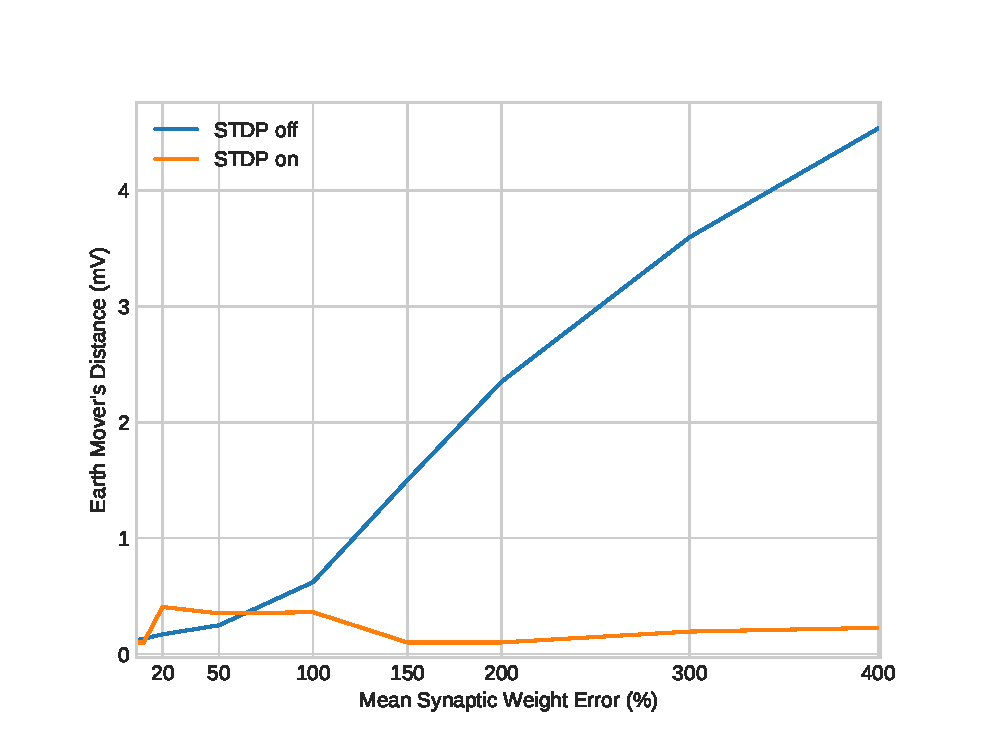
\includegraphics[width=0.8\linewidth]{figures/graphs/RESULT1.eps}
    \caption[Increase in EMD from inserting error in network synaptic weights]{Change in the Earth Mover's Distance between a baseline simulation and simulations with different levels of error applied to the synaptic weights between neurons.}
    \label{fig:RES1}
\end{figure}
\FloatBarrier


\subsection{The divergence over time from Gaussian error in synapse weights}

In order to determine the effect over time of applying gaussian error to all the
synaptic weights in a network, a network identical to that described in figure
\ref{fig:RES1TOP} was constructed and simulated with no error, and with 100\%
mean error. This was repeated with STDP on the weights in the network. 

The results, seen in figure \ref{fig:RES2} display considerable noise
distortion. However, within the noise distortion the trend demonstrates an
increase in observed divergence over time, while the divergence appears to
slightly decrease when simulating with STDP. While the results indicate the
aforementioned characteristics, the presence of noise in the output of this
experiment means that this trend is not supported as a conclusive deduction to
the exclusion of other interpretations, at least within the $2000ms$ runtime of
the simulation.

\begin{figure}[h!]
    \centering
    \addtolength{\leftskip} {-4cm}
    \addtolength{\rightskip}{-4cm}
    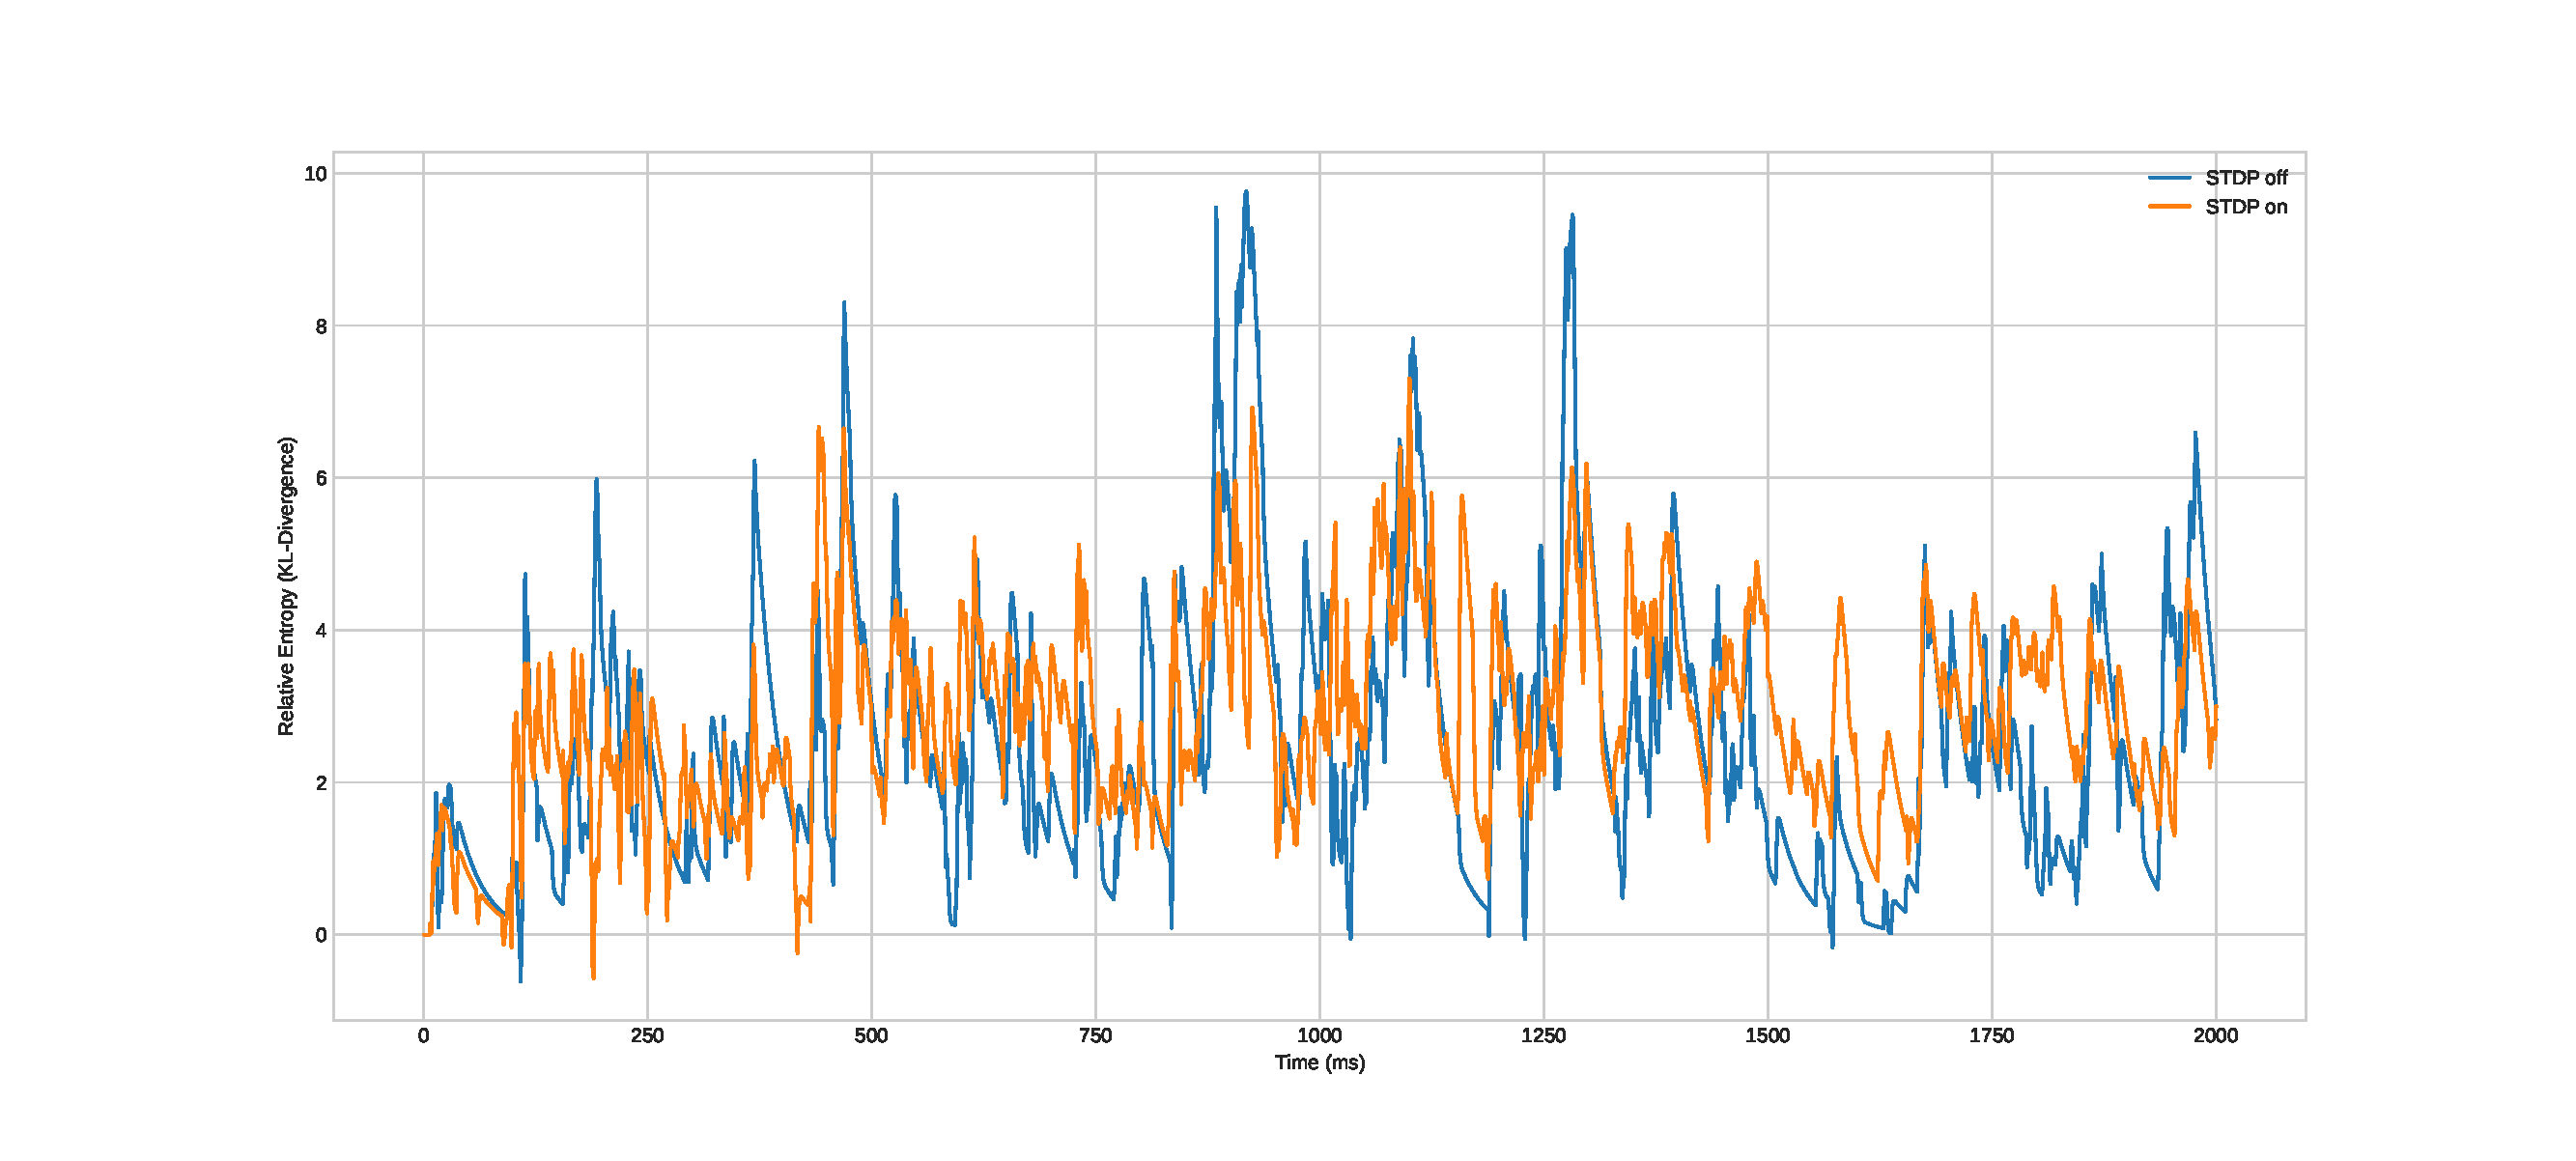
\includegraphics[width=1.6\linewidth]{figures/graphs/RESULT2.eps}
    \caption[Kullback-Leibler divergence over time]{The change in relative entropy over time measured as Kullback-Leibler divergence, where the mean weight error = 95\%. STDP in the simulation correlates to a slight reduction in divergence, however the divergence from millisecond to millisecond also seems to be be noisier with STDP.}
    \label{fig:RES2}
\end{figure}
\FloatBarrier

\section{Result evaluation}

The simulation developed and explained in this dissertation can be adapted to
show the effects of Gaussian error applied to synaptic weights that is
correspondent to measurement error produced in the brain imaging process. The
observed results when this error is applied therefore support the hypothesis
that measurement error both has an adverse effect on the accuracy of the
simulation of brain activity, and that this effect can be mitigated through the
application of synaptic plasticity.

The mitigation of measurement error through STDP suggests that a neural
network, simulated or otherwise, with synaptic plasticity should reach an
equilibrium state where weights change minimally over time, given the spiking pattern of the network remains consistent.

It is also worth noting that when calculating the difference between spiking
distributions the total accumulated potential, or the area under the curve,
should be the same for both distributions to ensure that the results were
comparable. This is true for both Kullback-Leibler divergence and Earth Mover's
Distance. However, due to the nature of the spiking pattern of the neurons, this
requirement of identical total accumulated potential
was not possible to guarantee. Future development would include investigations
to collect multiple comparisons for a given network, with the same measurement
error but different initial random seeds during simulation runtime. These
multiple results would provide data from which to calculate mean simulation
error, to be superimposed across result graphs.

\section{Reflection on development methodology}

In developing the software involved in this project, I took a reactive approach,
with the requirements of the software adapting as the results of experiments
took shape. This is substantially different from my original plan of identifying hard
requirements of the system and implementing them them all in a more traditional
"waterfall" development model. I found that it was much easier to let loose requirements set the direction of travel and
let experiments along the way determine the end result of the software.

The success of this experimental approach is partially due to an initial lack of
knowledge around the problem domain. As I understood more about computational
neuroscience, domains that seemed simple took on additional complexity, while
previously intractable concepts became apparent. Another benefit of taking an experimental and incremental approach to the
development of the project is that tasks naturally break down into small and
meaningful sections; each new piece of code does the correct amount of work to
solve a set purpose. Separating code into conceptual units in this manner aided
in readability when returning to them later to add or extend features.

The caveat to the experimental software development approach is that it does not
lend itself to a holistic system design or consistent architecture. When
defining and writing new data experiments, the flexibility of decoupled
components is ideal, but new code tends to be purpose built and highly coupled.
This would sometimes mean re-writing code several times as previously finished
code had new requirements.

By way of conclusion regarding development methodology, I’ve found that getting
development methodology right is both hard and a misnomer of sorts. It depends
on the project, the team if you have one, and the workload: what “right” means
will change as the code-base and requirements change. As these mature, the
project development moves from an experimental development cycle to one with
well formed requirements. As such, one solid way of working throughout a project
will cause friction later on, while flexibility to change how software is
developed as it evolves will improve the developer experience immensely. A lot
of time and effort both inside and out of the software development industry is
spent defining `Agile ways of working' \autocite{spolsky_you_2006}, however,
from my experiences on this project, it is better to be flexible and reject
workflow rigidity.

% Flexibility in ways of working does have its drawbacks however; deadlines must
% be set and adhered to throughout a project lest one finds themselves overworked
% and unable to produce outcomes that matter externally. In this aspect, my
% project would have benefited greatly from a larger sense of responsibility to
% myself and the targets I set myself at the beginning of the year. By way of
% example, I had originally planned that certain stages of my project could
% overrun safely, while others must be completed on time. Sticking to this plan
% was far harder than I originally anticipated, and in hindsight it would have been
% wise to re-scope the project as soon as it was clearly the best course of action,
% instead of carrying a metaphorical weight that it was clear couldn't reach the
% finish line.

\newpage

\section{Evaluation of dissertation objectives}

\subsubsection{Analyse and compare three published neural simulation packages.}
A selection of popular and notable simulation software packages and libraries are evaluated in section \ref{availableneuralsim} in this document. This evaluation was crucial to defining the specifications for this project's software development.

% This objective was met through the research in SECTION 2 through
% researching games, films and other projects as case studies. Interviews and
% correspondence with experts in the industry also competed the task.

\subsubsection{Identify the experiments that should be performed to determine
      the relation between measurement error in data from imaging a brain, and
      the performance of a neural simulation of such data.}
In section \ref{TheeffectofGaussianerror}, the weighting of synapses between neurons was identified as the property of the network that should be modified to order to emulate measurement error. The various methods that can be used to measure simulation performance are outlined in section \ref{Comparingspikingpatternsbetweentwonetworks}.

\subsubsection{Identify the requirements and features that the simulation
      tooling should implement to be capable of performing the project
      experiments.}
The requirements for the simulation software package described by this dissertation are defined in section \ref{SimulationRequirements}. These requirements were identified through the research outlined in the Literature Review, chapter 2.

\subsubsection{Identify the parameters in a brain simulation that can be
      modified during the simulation to emulate the measurement error of
      uploading the human brain.}
Following the research in the literature review, specifically section \ref{imagingresearch}, the value of the weights on synapses between neurons was identified as an appropriate approximation for measurement error that would occur in imaging the brain. 

\subsubsection{Analyse the performance of simulations that diverge with
      different measurement errors from a starting simulation.}

The differences in performance between diverging simulations that emulate differing levels of measurement error are analysed in \ref{Testingthesimulation}, and future work on this subject could readily expand this investigation to cover further parameters that affect performance.

\chapter{Ethical Considerations for Brain Simulation}
\setlength{\epigraphwidth}{0.4\textwidth}
\epigraphhead[50]{\epigraph{\large{`I ache, therefore I am.'}}{- Marvin the
      Paranoid Android\\
      Hitchhiker's guide to the galaxy\\ by Douglas Adams}}

In "Taking superintelligence seriously: Superintelligence: Paths, dangers,
strategies", Nick Bostrom argues that while the desirability of enhancing human
capacities, such as potential gains in life-span, cognition, and emotional
intelligence may be enticing, pursuit of this goal is not without danger.
\autocite{bostrom_superintelligence_2014}

The closer that society gets to primitive brain emulation, the more vital it
will become that we understand the moral and ethical implications of brain
emulation, such that the non-biological might gain sentience. A fully emulated
brain, imaged and simulated from its original chemical state, would surely be
subject to all the same thoughts, processes and emotional states as it did
pre-simulation. Indeed, if one desires to predict the future brain activity of a
living being, then it is necessary to leave every facet of the human psyche
intact. Therefore it is necessary to contemplate feeling and pain in a simulation.

\section{Pain and suffering in brain simulation}

If one assumes that it is both computationally possible to emulate the human
brain, and that true emulated emotion is as valid as human emotion,
then it follows that an emulated brain would be capable of both feeling and
understanding pain as we know it. Furthermore, a simulation capable of greater
cognition and intelligence than a human would also be capable of pain beyond
human comprehension; our perceptions of the world or indeed, the universe, are a
consequence of our neural biology \autocite{eagleman_human_2008}, and therefore
a simulation of greater or differing cognitive power to us may well experience
the universe and the concept of "being" differently, and possibly in a hightened
manner. With this in mind, it is worth defining the potential
causes of suffering in brain simulations. According to Ziesche and Yampolskiy,
these sources of suffering can be defined broadly as:

\begin{itemize}
    \itemsep-0.2em
    \item The transferred human mind intentionally suffers
    \item The transferred human mind unintentionally suffers
    \item Suffering occurs as a natural consequence of the actions or
    environment of the simulated mind
\end{itemize}
\autocite{ziesche_no_2019-1}.

The second of these, that the transferred mind may suffer unintentionally, is
the item of greatest interest to this dissertation. Unintentional suffering
could occur as a result of misconfiguration in simulation parameters, or error
produced during the course of mind transfer. 

Assuming that the simulation itself is not a source of pain, error produced when
transferring the human mind to a simulation could potentially damage the brain's
connections to the point of the simulation having a different personality, as
can happen with brain damage today, particularly in children and young
adolescents \autocite{max_personality_2015}. An intelligent simulation of a
human would understand that it had been unsuccessfully copied, itself an
unpleasant and likely traumatising realisation.

Finally, there is the possibility of an incorrect simulation or mind-transfer
simply going wrong during simulation, and abnormal brain activity being
simulated. While this would most likely become random meaningless data, it is
possible that such an error could effectively emulate a the mind
experiencing a seizure for as long as the simulation runs. 
 
\section{The rights of a simulation}

In order to prevent unintentional simulation failure causing suffering, fail-safe
mechanisms should be implemented such that simulated activity that is analogous
to a seizure or other abnormally excessive or synchronous neuronal activity
would terminate simulation after a timeout. This timeout should not exceed more
than an order of minutes of simulated time. In practice such a fail-safe
would require that the simulation is monitored at runtime, where such monitoring
may be objectionable for the sake of privacy, should simulated consciousnesses
care for privacy as we understand it.

Given a simulation that holds limited computational power, where the emulated
mind is no more cognitively able than a human, it would not be moral to simulate
such a sentient artificial intelligence with nothing to do, as boredom and
loneliness can be intensely negative and painful
\autocite{hawkley_loneliness_2010}. Thus, a simulation should peacefully turn
off or enter into a sleep-like state when there are no sensory inputs.

An emulation of a human mind should either exist as an original being, where
imperfections in the mind-uploading process are irrelevant, or as a perfect copy
of an existing mind, where the artificial intelligence is considered to be the
continuation of a person. The legal implications of this would be far reaching,
and are out of the scope of this discussion.


% \section{Kinder artificial intelligence}
% probably could go in conclusion. Cite lesswrong dude.
% https://wiki.lesswrong.com/wiki/Friendly_artificial_intelligence

% Is a brain simulation alive? 
% If accurate enough, how separable is a human and a brain simulation from that human?
% Is it ethical to allow a brain simulation to feel pain? 